\documentclass{tikzstandalone}
\begin{document}
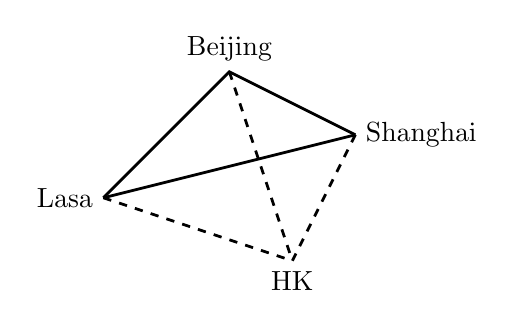
\begin{tikzpicture}[scale=.8,line width=1pt] % ,decoration={random steps, amplitude=.5pt,segment length=15pt}]
  % axes
  %\draw[help lines] (-1,0) grid (4,2);
  \coordinate [label=left:Lasa] (Lasa) at (0,0);
  \coordinate [label=below:HK] (HK) at (3,-1);
  \coordinate [label=above:Beijing] (Beijing) at (2,2);
  \coordinate [label=right:Shanghai] (Shanghai) at (4,1);
  \draw (Lasa) -- (Beijing) -- (Shanghai);
  \draw (Shanghai) -- (Lasa);
  \draw [dashed] (Lasa) -- (HK);
  \draw [dashed] (Beijing) -- (HK);
  \draw [dashed] (Shanghai) -- (HK);
\end{tikzpicture}
\end{document}